\chapter{Application to HCP pre-processing pipelines}

\section{Data}
\paragraph{HCP Data Acquisition}
The data was acquired from Human Connectome Project\footnote{\url{https://db.humanconnectome.org}}. We used the subjects 101006, 101017, 101410, 104820 and 105216. All these subjects were scanned using the HCP3T type of scanner. Figures \ref{fig:subject_details} and \ref{fig:subject_scan_details} gives more insight about the HCP subjects that were used for our study. 

\begin{center}
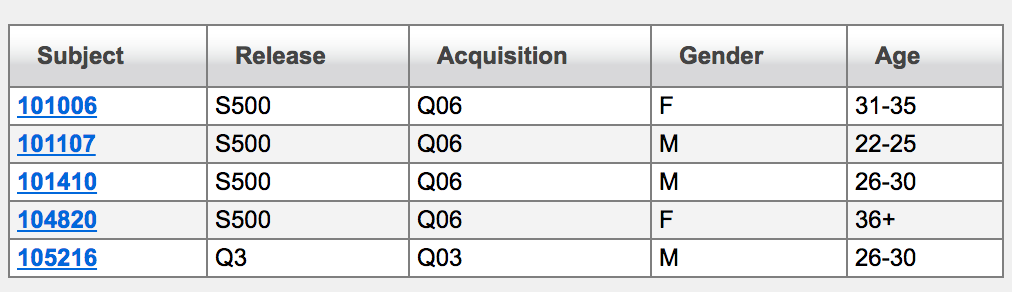
\includegraphics[width=\linewidth]{subjects_details.png}
\captionof{figure}{Subject Details}
\label{fig:subject_details}
\caption*{Extracted from \cite{DBConnectomeSite}}
\end{center}

\begin{center}
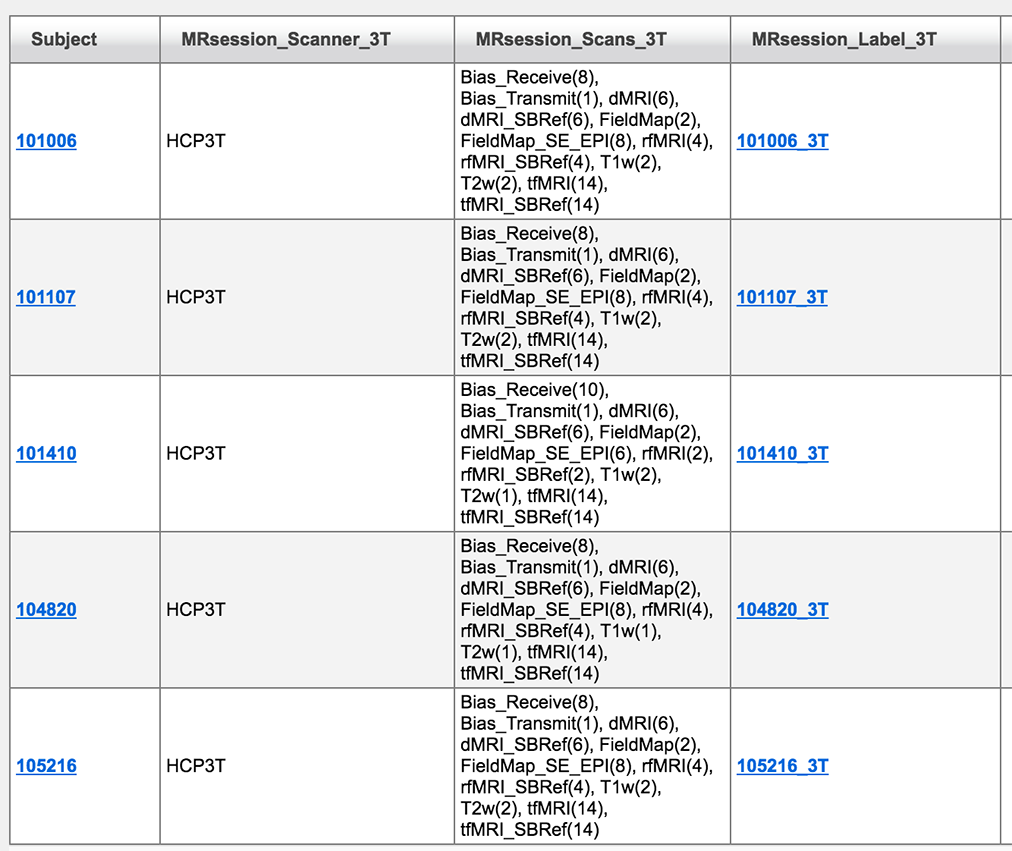
\includegraphics[width=\linewidth]{subject_scan_details.png}
\captionof{figure}{Subject Scan Details}
\label{fig:subject_scan_details}
\caption*{Extracted from \cite{DBConnectomeSite}}
\end{center}

\section{Processing}
\begin{itemize}
  \item PreFreeSurfer
  \item FreeSurfer
  \item PostFreeSurfer
  \item fMRIVolume
\end{itemize}

\section{Evaluation}
\paragraph{File comparision across conditions using metrics}
\begin{itemize}
  \item NRMSE
  \item Dice
  \item Checksum
  \item Hardware
\end{itemize}
